\documentclass[11pt,a4paper]{article}
\usepackage[utf8]{inputenc}
\usepackage[T1]{fontenc}
\usepackage{amsmath}
\usepackage[usenames,dvipsnames,svgnames,table]{xcolor}
\usepackage[normalem]{ulem}
\usepackage[left=1.00cm, right=1.00cm, top=0.40cm, bottom=0.2cm]{geometry}
\PassOptionsToPackage{defaults=hu-min}{magyar.ldf}
\usepackage[magyar]{babel}
\usepackage{framed, fancyhdr, wasysym, graphicx, multirow}

\begin{document}
\renewcommand{\labelitemi}{\textbullet}
\def\br{\\[0.1cm]}
\thispagestyle{empty}
\begin{center}
	\colorbox{lightgray}{{\large JPSMA3} \hspace{3cm} {\large Eseményvezérelt alkalmazások 2 3. beadandó} \hspace{5cm} \thepage}
\end{center}
\begin{framed}
	\begin{flushleft}
		{\large \textbf{Bauer Bence}}
		\hspace{3cm}{\large \textbf{3.Beadandó/19.Feladat}}
		\hspace{5.4cm}{\large 2018.12.13.}\br
		{\large JPSMA3}\br
		{\large bauerbence5@gmail.com}
	\end{flushleft}
\end{framed}
\section{Feladat}
Készítsünk programot, amellyel a potyogós amőba játékot lehet játszani, vagyis
az amőba azon változatát, ahol a jeleket felülről lefelé lehet beejteni a
játékmezőre. A játékmező itt is $nxn$-es tábla, és ugyanúgy X, illetve O jeleket
potyogtathatunk a mezőre. A játék akkor ér véget, ha betelik a tábla (döntetlen),
vagy valamelyik játékos kirak 4 egymás melletti jelet (vízszintesen, vagy átlósan).
A program minden lépésnél jelezze, hogy melyik játékos következik, és a tábla
egy üres mezőjére kattintva helyezhessük el a megfelelő jelet. Természetesen
csak a szabályos lépéseket engedje meg a program.
A program biztosítson lehetőséget új játék kezdésére a táblaméret megadásával
$(10 x 10, 20 x 20, 30 x 30)$, játék szüneteltetésére, valamint játék mentésére és
betöltésére. Ismerje fel, ha vége a játéknak, és jelenítse meg, melyik játékos
győzött (a táblán jelölje meg a győztes 4 karaktert). A program folyamatosan
jelezze külön-külön a két játékos gondolkodási idejét (azon idők összessége, ami
az előző játékos lépésétől a saját lépéséig tart, ezt is mentsük el és töltsük be).
\section{Elemzés}
\begin{itemize}
	\item A játékot tetszőleges méretű pályán játszhatjuk, melyet az ablak tetjén lévő
	mezővel tudunk beállítani, az "Új játék" gomb lenyomásával új játék indul az
	éppen a mezőben lévő pályamérettel.
	\item A feladatot egyablakos asztali alkalmazásként Windows Presentation Foundation grafikus felülettel
	valósítjuk meg.
	\item Az ablakon elhelyezünk egy File menüt (Mentés, Betöltés, Kilépés), Új játék
	beállítására szolgáló vezérlőt valamint egy státuszsort, mely a játékosok idejét és
	az éppen soron lévő játékost jelzi.
	\item A játéktáblát egy $nxn$-es nyomógombokból álló rács reprezentálja. Egy
	nyomógombra való kattintás hatására a kattintott mezőben megjelenik az éppen soron lévő játékos karaktere.
	\item A játék automatikusan feldob egy ablakot ha véget ért Döntetlen/Nyertes játékos
	nevével, valamint a két játékos idejével.
	\item A játék állapota adatbázisba menthető az Entity Framework ORM keretrendszer
	használatával. A betöltést és a mentést egyedi dialógusablakokkal végezzük, a mentések
	egyedi nevét a felhasználó adja meg.
\end{itemize}
\begin{figure}[h]
\centering
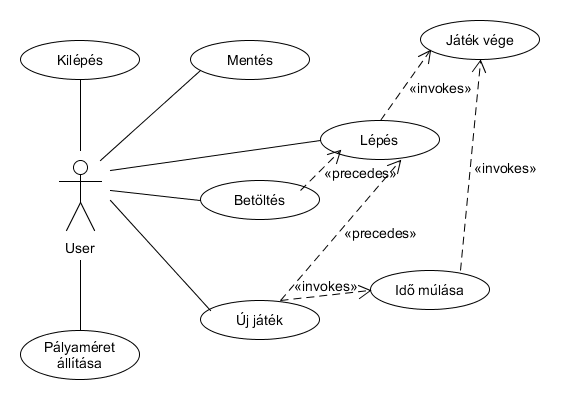
\includegraphics[width=11cm]{UMLs/UseCase.png}
\caption{Felhasználói eset diagram}
\end{figure}
\newpage
\thispagestyle{empty}
\begin{center}
\colorbox{lightgray}{{\large JPSMA3} \hspace{3cm} {\large Eseményvezérelt alkalmazások 2 3. beadandó} \hspace{5cm} \thepage}
\end{center}
\section{Tervezés}
\begin{itemize}
	\item Programszerkezet: A programot MVVM architektúrában valósítjuk meg:
	\begin{itemize}
		\item Modell: \textbf{Model}
		\item Megjelenítés: \textbf{View}
		\item Nézetmodell: \textbf{ViewModel}
		\item Perzisztencia: \textbf{Persistence}
	\end{itemize}
	\item A program környezetét az alkalmazás osztály \verb|App| végzi, amely példányosítja a
	modellt, a nézetmodell és a nézetet, biztosítja a kommunikációt, valamint felügyeli az
	adatkezelést.
	\item Csomagszerkezet:
	\begin{figure}[h]
		\centering
		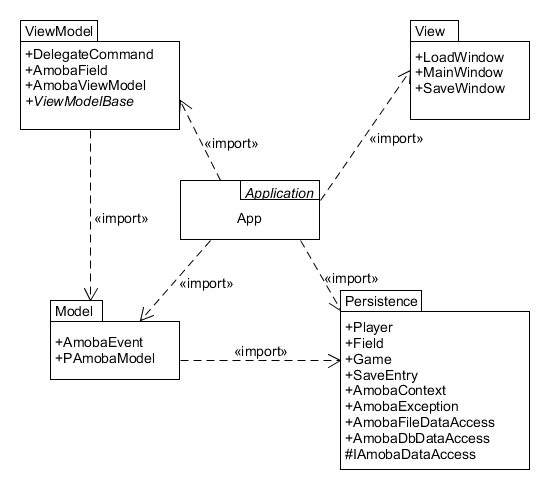
\includegraphics[width=10cm]{UMLs/Package.png}
		\caption{Csomagdiagram}
	\end{figure}
	\item Perzisztencia(3.ábra):
	\begin{itemize}
		\item Feladata a mentés és betöltés biztosítása.
		\item Az adattárolást az \textbf{IAmobaDataAccess} interfész biztosítja, továbba
		lehetőséget ad a játék állapotának mentésére(\textbf{SaveAsync})/
		betöltésére(\textbf{LoadAsync})	melyeket aszinkron módon végzünk.
		\item A szöveges fájl kezelésére az \textbf{AmobaFileDataAccess} osztályt vezetjük be.
		Ha hiba lépett fel a\\fájlkezelés során akkor azt \textbf{AmobaDataException}-el jelezzük.
		\item Az interfészt adatbázis alapú adatkezelésre az \verb|AmobaDbDataAccess| osztály
		valósítja meg. Az adatbáziskezelés az \textit{Entity Framework} használatával a
		\textbf{Field} és \textbf{Game} entitás típusokkal és az \textbf{AmobaContext}
		adatbázis kontextussal történik. A adatbáziskezelés során fellépő hibákat az
		\textbf{AmobaDataException} kivétel jelzi.
		\item A program az adatokat tehát tudja szöveges fájlként tárolni (melyek az \verb|sav|
		kiterjesztést kapják) vagy adatbázisban is (az \verb|App.config| konigurációs állományban
		megadott \textit{connection string} által leírt módon). Ezeket az adatokat a programban
		bármikor be lehet tölteni, illetve ki lehet menteni az aktuális állást.
		\item A játékosok kezeléséhez bevezetünk egy \textbf{Player} felsorolási típust, mely
		3 értéket vehet fel:\\ \textit{PlayerX, Player0, NoPlayer}.
	\end{itemize}
	\newpage
	\thispagestyle{empty}
	\begin{center}
		\colorbox{lightgray}{{\large JPSMA3} \hspace{3cm} {\large Eseményvezérelt alkalmazások 2 2. beadandó} \hspace{5cm} \thepage}
	\end{center}
	\begin{figure}[h]
		\centering
		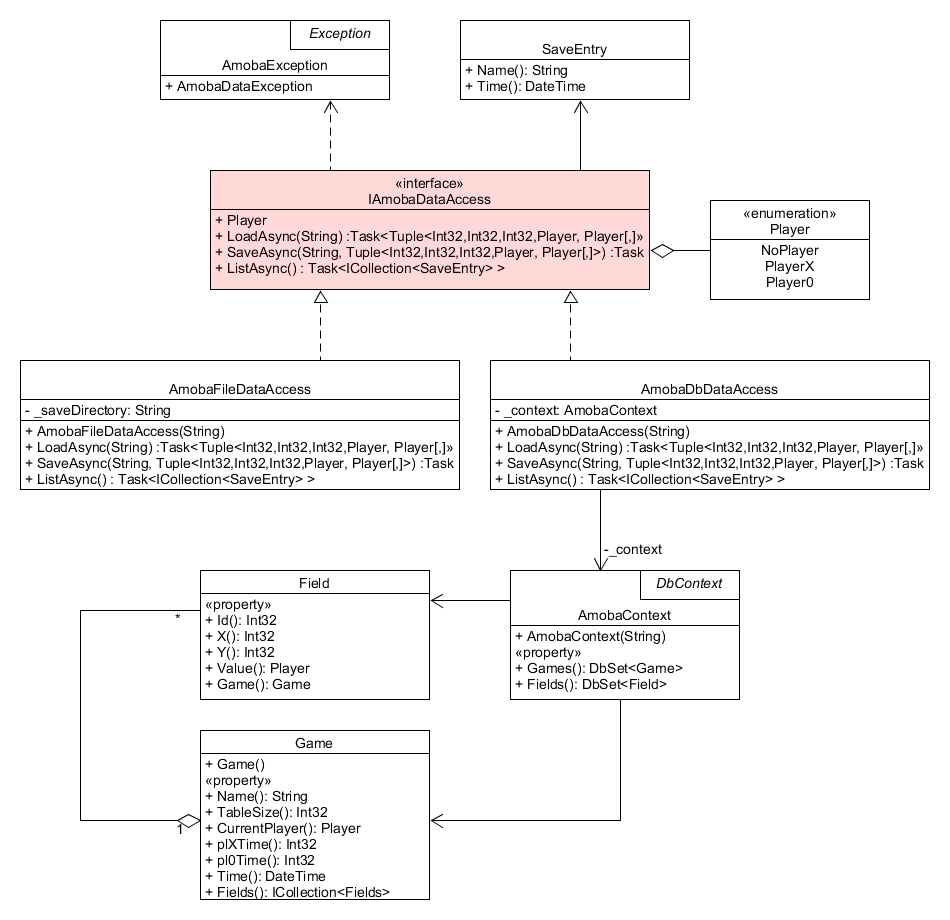
\includegraphics[width=17cm]{UMLs/PersistenceClass.png}
		\caption{A Persistence osztálydiagramja}
	\end{figure}
	\item Modell(4.ábra):
	\begin{itemize}
		\item A játék modelljét a \textbf{PAmobaModel} osztály valósítsa meg, ami figyeli
		a játékosok idejét\\(\textbf{playerXTime/player0Time}), a játék állását
		(\textbf{gameTable}), a soron lévő játékost (\textbf{\_currentPlayer})
		a lépések kezelését (\textbf{Step}), új játék kezdését (\textbf{NewGame}),\br
		lehet-e kattintani egy mezőre \textbf{(IsFieldActive)}
		valamint az idő telését is követi (\textbf{AdvanceTime}).
		\item Ha lépés történt akkor a model egy argumentum nélküli \textbf{Refresh}
		eseménnyel jelzi a \textit{Nézetmodell}-nek, hogy a játék állapota megváltozott.
		A játék újraírását (betöltés/új játék indítása) a \textbf{Reset} esemény jelzi.
		Ha a játék véget ért akkor azt egy \textbf{GameOver} eseménnyel jelzi, mely egy
		4 db \textit{Tuple}-ből álló tömböt (győztes mezők koordinátái), a 2 játékos
		idejét valamint a nyertes játékost adja át paraméterül.
		\item Példányosításkor megkapja az adatkezelés felületét, amellyel el tudja végezni
		a játék mentését (\textbf{SaveGame}), \\betöltését (\textbf{LoadGame})
		valamint a létező mentések lekérdezését (\textbf{ListGamesAsync}).
	\end{itemize}
	\newpage
	\thispagestyle{empty}
	\begin{center}
		\colorbox{lightgray}{{\large JPSMA3} \hspace{3cm} {\large Eseményvezérelt alkalmazások 2 3. beadandó} \hspace{5cm} \thepage}
	\end{center}
	\begin{figure}[h]
		\centering
		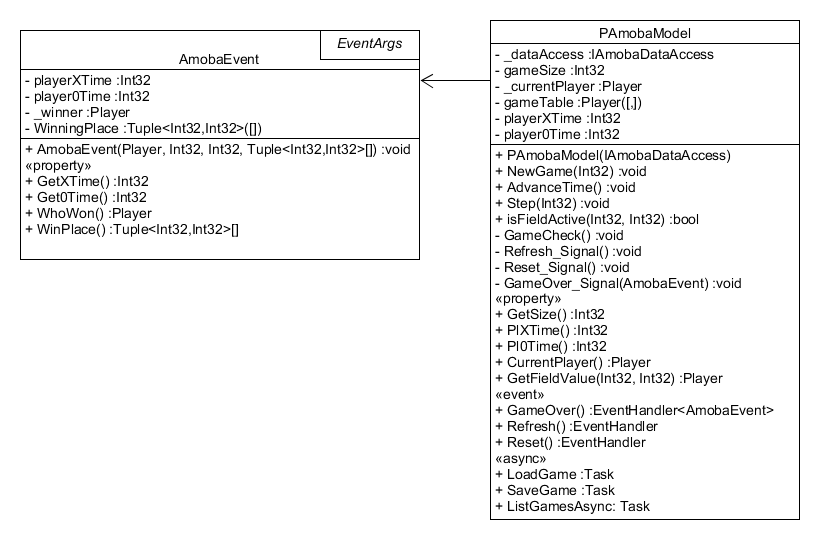
\includegraphics[width=17cm]{UMLs/ModellClass.png}
		\caption{Modell osztálydiagramja}
	\end{figure}
	\item Nézetmodell(5.ábra):
	\begin{itemize}
		\item A nézetmodell megvalósításához felhasználunk egy általános utasítás
		\textbf{(DelegateCommand)}, valamint egy ős változásjelző \textbf{(ViewModelBase)} osztályt.
		\item A nézetmodell feladatait az \textbf{AmobaViewModel} osztály látja el, amely
		parancsokat biztosít az új játék kezdéséhez, játék betöltéséhez,
		mentéséhez, valamint a kilépéshez. A parancsokhoz eseményeket kötünk,
		amelyek a parancs lefutását jelzik a vezérlőnek. A nézetmodell tárolja a
		modell egy hivatkozását \textbf{(\_model)}, de csupán információkat kér le tőle,
		illetve a játéktábla méretét szabályozza. Direkt nem avatkozik a játék
		futtatásába.
		\item A játékmező számára egy külön mezőt biztosítunk \textbf{(AmobaField)}, amely
		eltárolja a pozíciót, szöveget, klikkelhetőséget, szövegméretet, a mező benne van-e a
		4 nyertes mezőbe,\br valamint a lépés parancsát \textbf{(StepCommand)}.
		\item A mezőket egy felügyelt gyűjteménybe helyezzük a nézetmodellbe \textbf{(Fields)}.
	\end{itemize}
	\newpage
	\thispagestyle{empty}
	\begin{center}
		\colorbox{lightgray}{{\large JPSMA3} \hspace{3cm} {\large Eseményvezérelt alkalmazások 2 3. beadandó} \hspace{5cm} \thepage}
	\end{center}
	\begin{figure}[h]
		\centering
		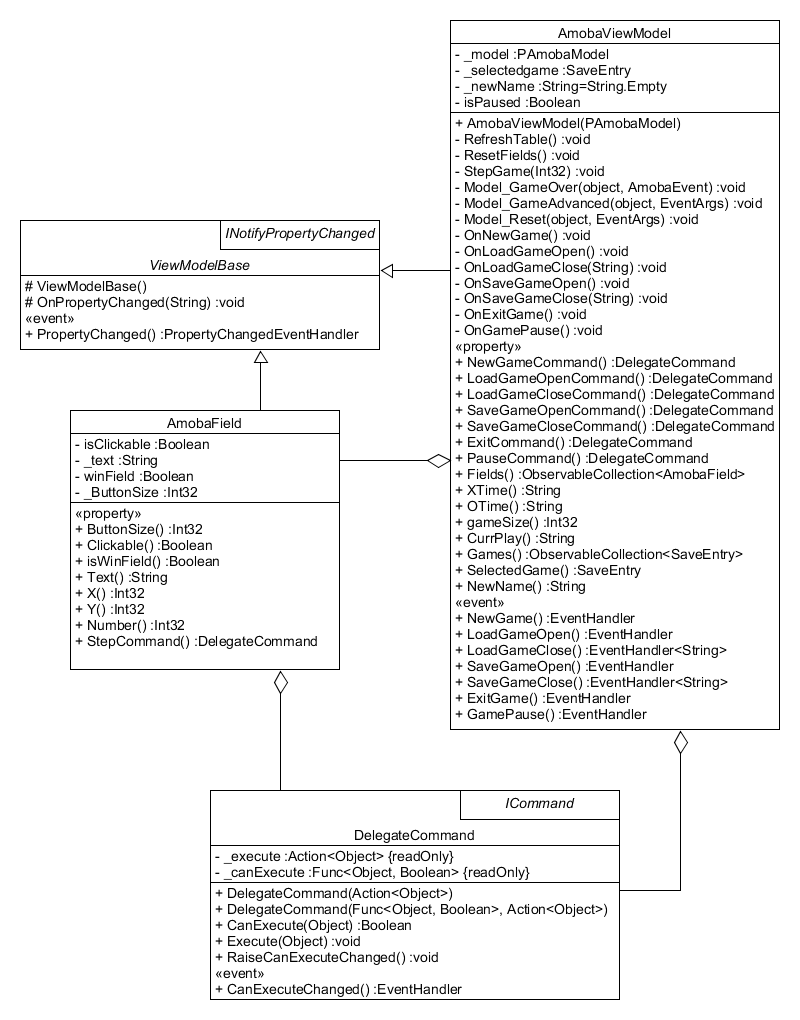
\includegraphics[width=17cm]{UMLs/ViewModell.png}
		\caption{Nézetmodell osztálydiagramja}
	\end{figure}
	\newpage
	\thispagestyle{empty}
	\begin{center}
		\colorbox{lightgray}{{\large JPSMA3} \hspace{3cm} {\large Eseményvezérelt alkalmazások 2 3. beadandó} \hspace{5cm} \thepage}
	\end{center}
	\item Nézet:
	\begin{itemize}
		\item A nézet csak egy képernyőt tartalmaz, a \textbf{MainWindow} osztályt. A nézet egy
		rácsban tárolja a játékmezőt, a menüt és a státuszsort. A játékmező egy
		ItemsControl vezérlő, ahol dinamikusan felépítünk egy rácsot
		\textbf{(UniformGrid)}, amely gombokból áll. Minden adatot adatkötéssel
		kapcsolunk a felülethez, továbbá azon keresztül szabályozzuk a gombok
		színét is.
		\item A betöltendő játékállapot bekérésért a \textbf{LoadWindow} osztály felel, amely
		dialógusablakként került megjelenítésre. A nézet egy \textbf{ListBox} vezérlőben
		listázza ki az elérhető játékállapotokat.
		\item Új mentésének nevét a \textbf{SaveWindow} osztály által megjelenített felület
		kéri be. A nézeten egy szövegdobozban \textbf{(TextBox)} megadható az új mentés neve,
		valamint a \textbf{LoadWindow} ablakhoz hasonlóan megjeleníti a létező mentések nevét
		(felülírás céljából).
		\item A figyelmeztető és információs üzenetek megjelenését beépített dialógusablakok
		segítségével végezzük.
	\end{itemize}
	\item Környezet (6. ábra):
	\begin{itemize}
		\item Az \textbf{App} osztály feladata az egyes rétegek példányosítása
		\textbf{(App\_Startup)}, összekötése, a nézetmodell, valamint a modell eseményeinek lekezelése,
		és ezáltal a játék, az adatkezelés, valamint a nézetek szabályozása.
		\item A játék léptetéséhez tárol egy időzítőt is \textbf{(\_timer)}, amelynek állítását is
		szabályozza az egyes funkciók hatására.
	\end{itemize}
	\begin{figure}[h]
		\centering
		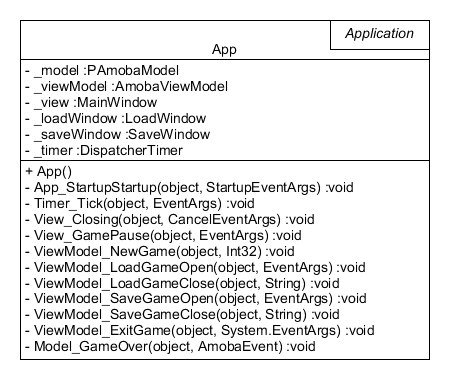
\includegraphics[width=11cm]{UMLs/App.png}
		\caption{A vezérlés osztálydiagramja}
	\end{figure}
\section{Tesztelés}
	\begin{itemize}
		\item A modell funkcionalitását egységtesztekkel vizsgáljuk az
		(\textbf{AmobaModelTest}) osztályban.
		\item Vizsgált esetek:
		\begin{itemize}
			\item\textbf{AmobaModel\_NewGameTest:} Új játék indításának tesztelése, mezők
			feltöltése.
			\item\textbf{AmobaModel\_StepTest:} Több lépés tesztelése, játékosváltás, illetve
			megfelelő karakterek \\ elhelyezése.
			\item\textbf{AmobaModel\_AdvanceTimeTest:} idő múlásának tesztelése, illetve, hogy
			az éppen soron lévő \\ játékos ideje telik-e.
			\item\textbf{AmobaModel\_GameOverTest:} Meghívódik-e a \textbf{GameOver} esemény
			ha egy játékos kirakja a \\ szükséges 4 karaktert.
			\item\textbf{LoadGameTest:} Játék betöltés tesztelése az interfészből
			származtatott mock objektummal.
		\end{itemize}
	\end{itemize}
\end{itemize}
\end{document}